

%\newpage
\section{Overview}

%Graph Neural Networks (GNNs) are powerful architectures that generalizes deep learning over graphs. However, GNNs are black-box machine learning models as they lack human-intelligible explanations of their predictions. 
%Owing to the popularity of GNNs in many applications, there is an increasing need to explain GNN predictions. Recently, there has been a significant amount of interest in explainability of GNNs. These explainability methods differ from each other on several aspects such as types of explanations, use of model information, and training procedures among others. We organize and categorize these methods to develop a deeper understanding of the existing works and provide a broad picture of their applicability in different scenarios. 


With the widespread adoption of GNNs across various applications, the demand for explaining their predictions has grown substantially. Recently, the community has witnessed a surge in efforts dedicated to the explainability of GNNs. These methods exhibit variations in terms of explanation types, utilization of model information, and training procedures, among other factors. We organize and categorize these methods to develop a deeper understanding of the existing works and provide a broad picture of their applicability in different scenarios.



\begin{figure*}[htbp]
  \centering
  \vspace{-.5mm}
  %\includegraphics[]{test3_schema.pdf}
  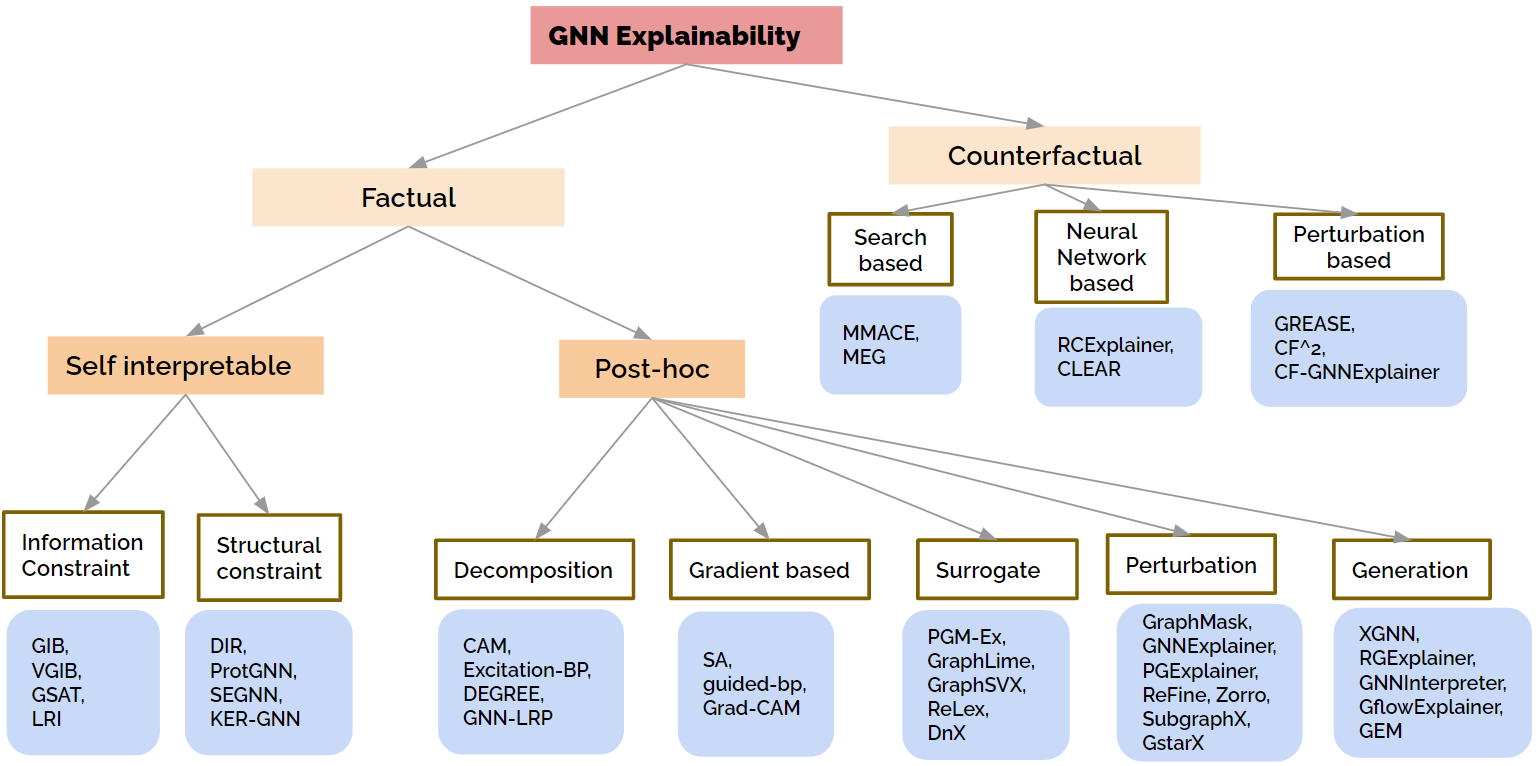
\includegraphics[width= .95\textwidth]{submissions/Sourav2023/Schema_V12.png}
  \centering
  \caption{\small \textbf{Overview of the Schema.} \textbf{(1) Factual.}  Information constraints: GIB \cite{GIB}, VGIB \cite{VGIB}, GSAT \cite{GSAT}, LRI \cite{inject-explain}; Structural Constraints: DIR \cite{D_invariant_rationale}, ProtGNN \cite{protgnn}, SEGNN \cite{SE-GNN}, KER-GNN \cite{kergnns}; Decomposition: CAM \cite{Excitation-BP}, Excitation-BP \cite{Excitation-BP}, DEGREE \cite{degree}, GNN-LRP \cite{GNN-LRP}; Gradient-based: SA \cite{guided-bp} , Guided-BP \cite{guided-bp} , Grad-CAM \cite{Excitation-BP}; Surrogate: PGM-Ex \cite{pgexplainer}, GraphLime \cite{graphlime}, GraphSVX \cite{graphsvx}, ReLex \cite{RELex}, DnX \cite{distilexplain}; Perturbation-based: GNNExplainer\cite{ying2019gnnexplainer}, GraphMask \cite{Graph-mask}, PGExplainer \cite{pgexplainer}, ReFine \cite{ReFine}, ZORRO \cite{zorro}, SubgraphX \cite{subgraphX}, GstarX \cite{gstarx}; Generation: XGNN \cite{xgnn}, RGExplainer \cite{RL-enhanced}, GNNInterpreter \cite{gnninterpreter}, GFlowExplainer \cite{Gflow}, GEM \cite{Gen-causal}; \textbf{(2) Counterfactual.} Search-based: MMACE \cite{agnostic-counter} , MEG \cite{meg-counter}; Neural Network-based: RCExplainer \cite{robust-counter}, CLEAR \cite{clear-counter}; Perturbation-based: GREASE \cite{chen2022grease}, CF2 \cite{cf^2-counter}, CF-GNNexplainer \cite{cfgnnex}
  }
  \label{fig:schema}
\end{figure*}


\noindent
\textbf{Main Schema: Factual and Counterfactual Methods. } Figure \ref{fig:schema} provides an overview of the broad categorization of the existing works. Based on the type of explanations, we first make two broad categories: (1) Factual and (2) Counterfactual. Factual methods aim to
find an explanation in the form of input features with the maximum influence over the prediction. These explanations can be a set of either node features or a substructure (set of nodes/edges) or both. On the other hand, counterfactual methods provide an explanation by finding the smallest change in the input graph that changes the model's prediction. Hence, counterfactual explanations can be used to find a set of similar features that can alter the prediction of the model.\\
\noindent
\textbf{Organization. }In the following sections, we describe each category in detail and provide summary of various explainability methods in each category. In Sec. \ref{sec:sourav_:Factual}, we describe the factual approaches which are further classified into self-interpretable and post-hoc categories. In Sec. \ref{sec:sourav_:Counterfactual}, the counterfactual methods are categorized into perturbation-based, neural network-based and search-based methods. Sec. \ref{sec:sourav_:Others} presents three special categories of explainers such as temporal, global and causality-based. In Sec. \ref{sec:sourav_:application}, we overview the explainer methods that are relevant for specific applications in different domains such as in social networks, biology, and computer security. Lastly, we review widely used datasets in Sec. \ref{sec:sourav_:datasets} and evaluation metrics in Sec. \ref{sec:sourav_:eval}.


% subgraph Given the input graph and the GNN model, the factual methods aim to find the smallest sub-graph that provides the same prediction as on the entire input graph.
%  In contrast, counterfactual methods aim to find minimal changes in the input graph that can alter the prediction of the model. In graphs, these perturbations usually correspond to addition and removal of the
% edges. We describe the works in individual categories in the following sections. \\\\




% \begin{figure}

% \includegraphics[bb= 1 150 600 700]{Schema_v2.png}

% \caption{}

% \end{figure}
\iffalse
\begin{table}[htbp]
\footnotesize
\begin{tabular}{|l  |c |   c|   c | c  |}
\hline

%          & (1)       & (2)       & (3)       & (4)       & (5)       \\ \hline
Pred Type & Categ1    & Categ2  & Categ3    & Methods    \\ \hline
 %         &           &           &           &           &           \\ \hline
\textbf{Factual}     & \textit{Post-hoc}    & White-box   & Decomposition  & \cite{GNN-LRP} \cite{Excitation-BP} \cite{co-operative}   \\ %\hline
                &     &    &   &      \\ \hline
        
            &   &   & Gradient-based  & SA\cite{guided-bp} Guided-bp\cite{guided-bp} Grad-CAM\cite{Excitation-BP} CAM\cite{Excitation-BP}     \\ %\hline
             &    &    &     &       \\ \hline \hline
             
       &      & Black-box    & Surrogate     &  \cite{graphlime} \cite{RELex} \cite{pgm-ex} \cite{distilexplain}         \\ %\hline
          &     &     &     &         \\ \hline
       &      &      & Perturbation      & \cite{ying2019gnnexplainer} \cite{pgexplainer} \cite{Graph-mask} \cite{subgraphX}  \cite{PAGElink}      \\ %\hline
          &     &     &    &         \\ \hline
       &      &      & Generation      & \cite{xgnn} \cite{RL-enhanced} \cite{Gen-causal} \cite{Gflow} \cite{gnninterpreter}        \\ %\hline
          &     &     &    &         \\ \hline \hline 
     & \textit{Self-interpretable}    & constraint-based   & information constraint  & \cite{GIB} \cite{VGIB} \cite{GSAT}  \cite{inject-explain} \cite{GCI}  \\ %\hline
                &     &    &   &       \\ \hline
     &    &    & Structural constraint  & \cite{SE-GNN}  \cite{D_invariant_rationale} \cite{protgnn} \cite{non-para-ex} \cite{structuralEx}  \\ %\hline
                &     &    &   &       \\ \hline \hline 
     &   & Parameter-based   &   & \cite{GCAN} \cite{kergnns}     \\ %\hline
                &     &    &   &       \\ \hline \hline \hline 
\textbf{Counterfactual}     &    &    & Perturbation  & \cite{cf^2} \cite{agnostic-counter}  \cite{cfgnnex} \cite{RC-ex} \cite{record-counter} \cite{meg-counter} \cite{MOO-counter} \cite{clear-counter} \cite{Global-counter}   \\ %\hline
                &     &    &   &       \\ \hline    
     &    &    & Neural Network  & \cite{}     \\ %\hline
                &     &    &   &       \\ \hline   
     &    &    & Search-based  & \cite{}     \\ %\hline
                &     &    &   &       \\ \hline  
         &    &    & Others  & \cite{}     \\ %\hline
                &     &    &   &      \\ \hline   
\end{tabular}
\caption{Overview of Schema }
\label{reg_mar_3_1_value}
\vspace{-5mm}
\end{table}

\fi



%We further classify the factual explainers into two types - 1) Self-interpretable and 2) Post-hoc based on integration of explainability architecture with the main model. The self-interpretable explainable methods design explainability architecture directly inside the model. Based on design of the explainability, we further classify the self-interpretable methods into two types - 1) constraint based and 2) Parameter based. If the design of the explainability architecture is based on constraints then we classify them as constraint based methods. Typically, two types of constraints are used - 1) Information constraints and 2) Structural constraint. However, if the design of explainability is based on using parameter of the model, we classify them as parameter based methods.   \\\\